% =====================================================================
% SECTION IV -- EXPERIMENTAL EVALUATION (style mirrors companion paper)
% =====================================================================
\section{Experimental Evaluation}
\label{sec:experimental_evaluation}

\raggedbottom

\subsection{Measured-Data Setup, Protocol, and Baselines}
\label{subsec:setup}

We evaluate ENCORE in closed loop on a $1$\,MW$_{\mathrm{IT}}$ liquid-cooled
hall; facility-level flexibility comes from aggregating halls, while hotspot
and condensation safety remain local. Every experimental input is measured
data; no synthetic disturbance process appears in this section. Heat-load
uncertainty comes from the Alibaba PAI GPU-cluster trace~\cite{weng2022mlaas}
($2.0$ million workers over $46$ usable days) mapped to a hall profile at
$5$-min resolution. Day-ahead heat forecasts use only information available
at the $12{:}00$ issue time: the survival-weighted load of jobs already
running plus an hour-of-day/level regression for short-job churn, both fit
causally. Weather is the Houston Intercontinental (KIAH) record paired with
\emph{archived} day-ahead numerical-weather-prediction (NWP) dew-point
forecasts,\footnote{Open-Meteo previous-runs archive,
\texttt{dew\_point\_2m\_previous\_day1}; measured day-ahead residual standard
deviation $2.0$\,K at this site. Prices and weather were accessed via
\texttt{gridstatus} and the Iowa Environmental Mesonet.} so both the
calibration and every simulated day use real forecast errors. Prices are
ERCOT day-ahead settlement-point prices, $15$-min real-time prices, and ECRS
clearing prices for the Houston hub.

The protocol separates design from validation. The trace is split into day
blocks: the first two thirds (fit block) calibrate forecasts, conformal sets,
and every design constant (gain $K$ with authority $300$\,kW/K, face
allocation $0.35/0.35/0.30$, $\epsd$); the final third (evaluation block) is
replayed exactly once, in closed loop, over ten 2024 ERCOT weeks spanning all
seasons (including Winter Storm Heather) $\times$ $20$ random seeds. All
participants in a seed face identical realized disturbances and activation
calls ($p_{\mathrm{act}}=0.15$, $d=30$\,min, $\gamma=2$). Offline
certification and offering for one day takes seconds on a desktop workstation
(Intel Core i9; no GPU), and every figure and table regenerates from
committed configurations and seeds by a single \texttt{make figures}.

Six participants are compared, spanning uncertified, stochastic, certified,
and alternative-resource designs:
\begin{enumerate}
\item \textbf{Idle}: the non-participating plant (B1); its trajectory defines
the baseline and absorbs workload-tail days that no market action causes.
\item \textbf{Deterministic envelope} (B2): offers $q_h = F(x,c_h)$ with no
uncertainty treatment; the upper bound any strategy can monetize, and the
cautionary case.
\item \textbf{Sample approximation} (B3): offers from a $20$-scenario
empirical box; stochastic but guarantee-free.
\item \textbf{ENCORE} (B4): offers from $\Ft$ with nested sets
($\epss{=}0.05$, $\epsd{=}0.3$).
\item \textbf{Battery} (B5): a stationary battery sized to the same hourly
energy, before capital cost.
\item \textbf{Curtailment} (B6): workload curtailment priced at a
quality-of-service cost.
\end{enumerate}
B2--B4 share the offering objective, settlement, and real-time machinery;
they differ only in the envelope they trust.

% --------------------------- TABLE II --------------------------------
\begin{table*}[t]
\centering
\caption{Closed-loop market performance over ten 2024 ERCOT weeks $\times$
$20$ seeds ($1{,}400$ day-seeds per participant, per MW of IT load). MV:
market value relative to Idle. Violations: hotspot day-seeds (maximum
excursion). Bold marks the best market value among participants with zero
violation episodes inside their stated domain.}
\label{tab:summary}
\setlength{\tabcolsep}{4pt}
\scriptsize
\begin{tabular*}{\textwidth}{@{\extracolsep{\fill}}llrrrrr}
\toprule
\textbf{Block} & \textbf{Method}
& \textbf{MV (\$/day)}
& \textbf{Committed (kW/day)}
& \textbf{Delivery ratio}
& \textbf{Penalty (\$/day)}
& \textbf{Violations: days (max K)} \\
\midrule
\multirow{6}{*}{Ten-week average}
& Idle (B1)            & $0.0$            & $0$    & --     & $0.00$ & 5 (0.25)$^{\dagger}$ \\
& Det.\ envelope (B2)  & $35.1 \pm 50.5$  & $388$  & $0.82$ & $1.49$ & $229$ ($9.8$) \\
& Sample approx.\ (B3) & $14.9 \pm 24.2$  & $126$  & $0.97$ & $0.25$ & $47$ ($4.9$) \\
& \textbf{ENCORE (B4)} & $\mathbf{10.6 \pm 15.7}$ & $54$ & $0.95$ & $0.17$
  & $\mathbf{0}$ \textbf{in-domain} ($1.6$) \\
& Battery (B5)         & $6.5 \pm 17.6$   & $616$  & $1.00$ & $0.00$ & $0$ \\
& Curtailment (B6)     & $25.6 \pm 35.8$  & $333$  & $1.00$ & $0.00$ & $0$ \\
\midrule
\multirow{6}{*}{Scarcity week (Heather)}
& Idle (B1)            & $0.0$             & $0$      & --     & $0.00$  & $0$ \\
& Det.\ envelope (B2)  & $221.9 \pm 337.5$ & $1{,}220$ & $0.77$ & $11.78$ & $57$ ($9.0$) \\
& Sample approx.\ (B3) & $113.7 \pm 166.8$ & $541$    & $0.93$ & $2.23$  & $15$ ($4.9$) \\
& \textbf{ENCORE (B4)} & $\mathbf{97.1 \pm 140.4}$ & $414$ & $0.92$ & $1.65$
  & $\mathbf{0}$ \textbf{in-domain} ($1.6$) \\
& Battery (B5)         & $76.5 \pm 126.4$  & $764$    & $1.00$ & $0.00$  & $0$ \\
& Curtailment (B6)     & $166.2 \pm 255.5$ & $871$    & $1.00$ & $0.00$  & $0$ \\
\bottomrule
\multicolumn{7}{l}{\footnotesize $^{\dagger}$Exogenous summer workload-tail
days exceeding the plant's sizing with no market participation; identical for
B4.}
\end{tabular*}
\vspace{-5mm}
\end{table*}

\vspace{-3mm}
\subsection{The Certification Wall and the Value of Information}
\label{subsec:wall}

Fig.~\ref{fig:F1}(a) sweeps the certified offer against residual workload
volatility (Borg-2019~\cite{tirmazi2020borg} residuals scaled by $\kappa$;
dry day, hour $14$, $d=30$\,min). Certification is volatility-limited: the
product holds a ${\sim}125$\,kW plateau per MW of IT load up to
$\kappa\approx 0.5$, then falls through $92$ and $50$\,kW to zero at the full
mixed-batch volatility $\kappa=1$. The binding statistic is not burst
amplitude but \emph{sustained hourly residual energy}: deviations persisting
for tens of minutes consume exactly the buffer the product sells, which is
why the energy face of \eqref{eq:box} dominates the margins.

The markers place the \emph{real} PAI hall on this wall at two day-ahead
information levels. With a climatology forecast, its conformal sets certify
$40.7$\,kW; the job-aware forecast, which uses only the running-job state the
operator already possesses at the deadline, shrinks held-out residual energy
by $19\%$ and lifts the certified offer to $74.6$\,kW ($+83\%$). Day-ahead
workload information is not an accuracy nicety: it moves a hall along the
certification wall, and pricing that movement is precisely what a
context-dependent envelope is for. Fig.~\ref{fig:F1}(b) shows the weather
coupling on the same hall: the conditional envelope degrades smoothly with
the NWP dew-point forecast, while a context-free certificate must assume the
worst hour and forfeits most of the dry-day capability. This is the
market-layer counterpart of context-adaptive robustness in
control~\cite{shen2026cdro}.

\begin{figure*}[t]
\centering
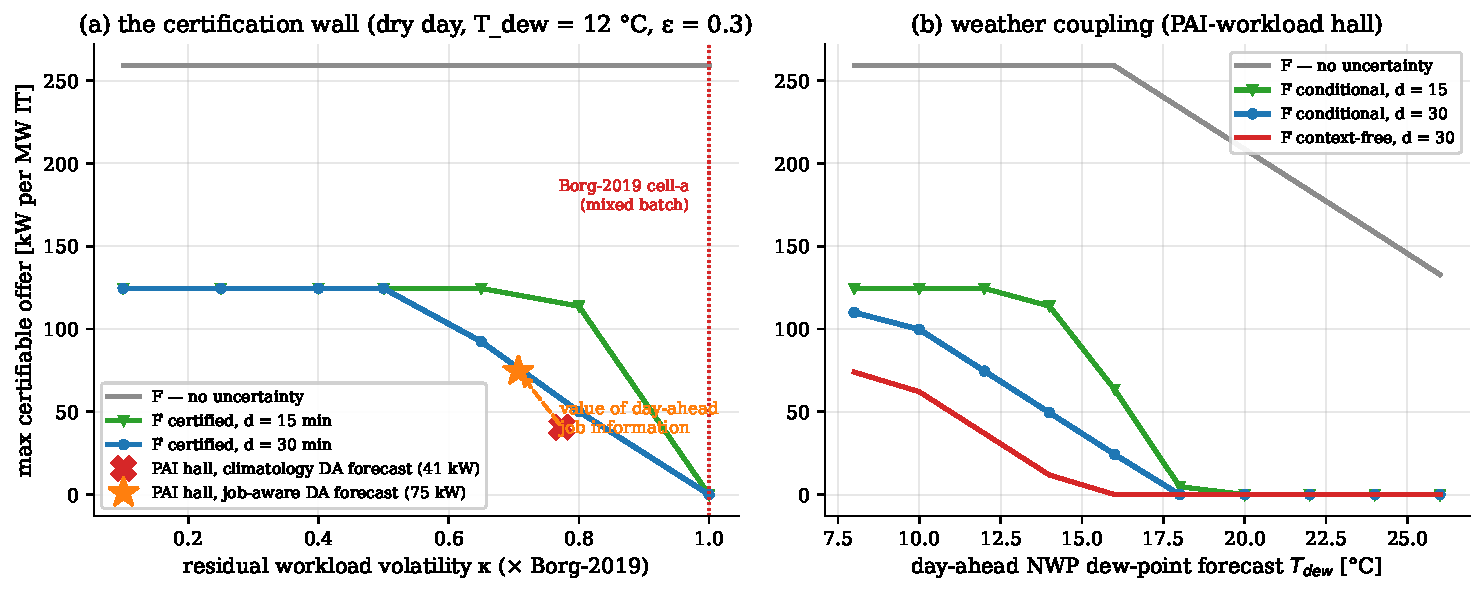
\includegraphics[width=\textwidth]{../results/phase6/F1_context.pdf}
\caption{The certified envelope on measured data ($d=30$\,min,
$\epsd=0.3$, $\epss=0.05$). (a)~Certified offer vs.\ residual workload
volatility ($\times$ Borg-2019 cell-a); markers: the real PAI hall under
climatology vs.\ job-aware day-ahead forecasts ($40.7\to 74.6$\,kW). (b)~Weather coupling: conditional vs.\
context-free certification vs.\ the deterministic ceiling, against the real
day-ahead NWP dew-point forecast.}
\label{fig:F1}
\vspace{-2mm}
\end{figure*}

\vspace{-3mm}
\subsection{Ten-Week Closed-Loop Market Results}
\label{subsec:market}

Table~\ref{tab:summary} aggregates $1{,}400$ controller-days per participant.
Three observations order the comparison.

\emph{1) Safety is the product.} The deterministic envelope monetizes the
most capacity ($\$35.1$/day per MW of IT load) but violates the hotspot limit
on $229$ of $1{,}400$ day-seeds, by up to $+9.8$\,K: on real workload weeks an
uncertified envelope is not a flexibility product but deferred downtime.
ENCORE commits $8\times$ less capacity, monetizes $\$10.6$/day, and incurs
\emph{zero} violation episodes inside its certified domain. Its ten
beyond-domain excursions are statistically expected, since the safety set is
calibrated at $1-\epss=95\%$; they stay below $1.6$\,K, where hardware
frequency scaling is the designed backstop, versus B2's $9.8$\,K. The sample
approximation lands between ($47$ violation day-seeds, up to $4.9$\,K): the
gap is the guarantee, not the stochastic modeling.

\emph{2) Value concentrates where the grid needs it.} The scarcity block of
Table~\ref{tab:summary} carries the economics: ENCORE commits
$414$\,kW/day and earns $\$97$/day per MW of IT load during Winter Storm
Heather, about $44\%$ of what even the unconstrained B2 monetizes there,
with $1{/}7$ of its penalty exposure and none of its violations. Averaged
over all ten weeks the certified value is $\$10.6$/day
(${\approx}\$3.9$k/MW-yr): 2024 ERCOT capacity prices outside scarcity hours
are a few dollars per MWh, so the ceiling for \emph{any} strategy is B2's
$\$35$. Cooling-side flexibility is a scarcity asset, which is the correct
shape for a resource whose marginal cost is thermal risk.

\emph{3) Zero capital, zero workload impact.} Scaled to a $100$\,MW campus,
the certified product is worth ${\approx}\$390$k/yr using hardware the
facility already owns. The battery returns less ($\$6.5$/day) before its
capital cost is counted; curtailment returns more ($\$25.6$/day) but prices
direct interference with the compute product, which the cooling side never
touches. The two are portfolio complements; only the cooling loop is free.

Fig.~\ref{fig:portfolio} resolves Table~\ref{tab:summary} by week in the
value--safety plane. Every participant's weekly cloud sits on a frontier
whose horizontal axis is paid in violations: the deterministic envelope buys
its value at up to $9.8$\,K of excursion, the sample approximation at up to
$4.9$\,K, while ENCORE's cloud is pinned to the safe axis with the scarcity
week as its high-value outlier. The certified product is the only
cooling-side participant whose position an operator can accept without
re-deriving the risk case week by week.

\begin{figure}[t]
\centering
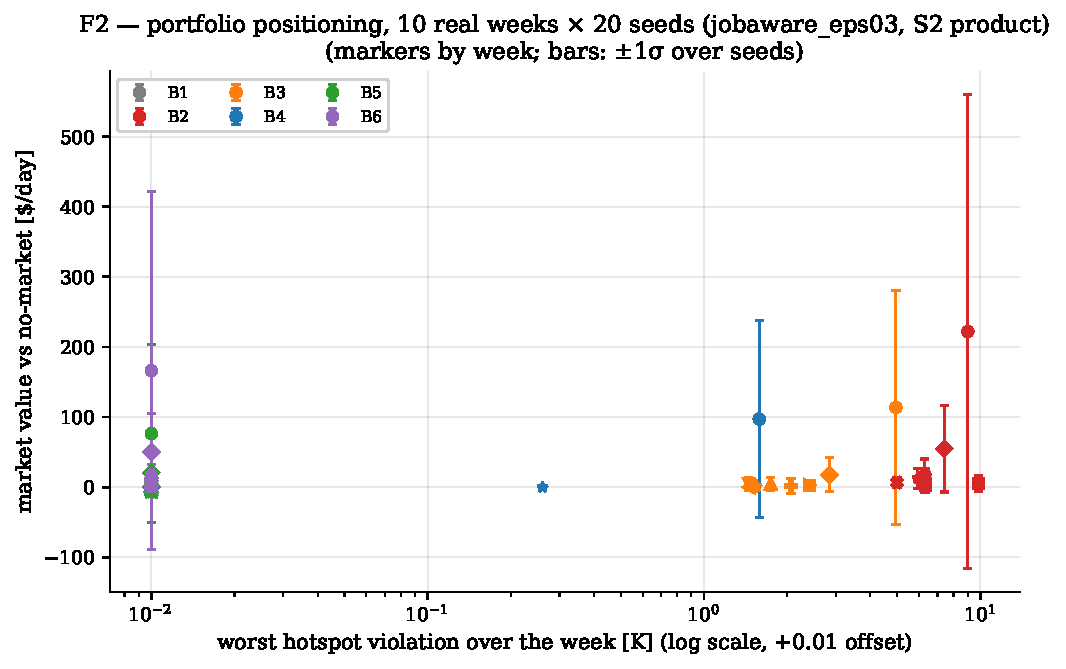
\includegraphics[width=\columnwidth]{../results/phase6/F2_portfolio_jobaware_eps03.pdf}
\caption{Weekly market value vs.\ maximum hotspot excursion over ten weeks
$\times$ $20$ seeds (markers: weeks; bars: $\pm 1\sigma$ over seeds).}
\label{fig:portfolio}
\vspace{-3mm}
\end{figure}

\vspace{-3mm}
\subsection{Certificate Validation}
\label{subsec:cert}

Theorem~\ref{thm:main} makes two falsifiable claims; the held-out replay
tests both at the design point $\epsd=0.3$.

\emph{Safety clause.} Across $1{,}400$ day-seeds, no violation episode starts
in an hour whose realized disturbance lies in $\Wsafe(c)$: zero in-domain
episodes, matching clause (i) on its stated domain. The ten beyond-domain
episodes are bounded by $1.6$\,K.

\emph{Delivery clause.} Of $122$ activated obligations at the design point,
$24$ fell short ($19.7\%$, within the priced budget $\epsd=0.3$); every
failure is attributable to a warm start at the envelope boundary covered by
the ball of Lemma~\ref{lem:e0}, and none occurred on a cold start with
in-set disturbances ($0$ of $22$; exact $95\%$ Clopper--Pearson upper bound
$15.4\%$). Table~\ref{tab:frontier} reports the $\epsd$ frontier: the
conservative point certifies less depth and fails less often, the design
point monetizes more and pays more penalty, and both stay within their stated
budgets. The frontier is the product-design freedom that the nested
construction \eqref{eq:nested} creates: $\epsd$ moves along it while the
safety clause is untouched.

% ---- Table: eps_d frontier ----
\begin{table}[t]
\centering
\caption{The delivery-risk frontier on the held-out replay (ten weeks
$\times$ $20$ seeds; safety set fixed at $\epss=0.05$).}
\label{tab:frontier}
\setlength{\tabcolsep}{4pt}
\scriptsize
\begin{tabular}{lcc}
\toprule
 & $\epsd=0.1$ & $\epsd=0.3$ (design) \\
\midrule
Market value (\$/day per MW) & $9.1$ & $10.6$ \\
Committed (kW/day) & $43$ & $54$ \\
Obligations / failures & $118$ / $15$ & $122$ / $24$ \\
Observed failure rate vs.\ budget & $0.127 \le 0.1{+}$CI & $0.197 \le 0.3$ \\
Cold-start failures (CP$_{95}$ bound) & $0$ ($\le 0.137$) & $0$ ($\le 0.154$) \\
In-domain safety episodes & $0$ & $0$ \\
\bottomrule
\end{tabular}
\vspace{-3mm}
\end{table}

\emph{Warm-start accounting.} Because the offering maximizes value, the
chosen $q_h$ sits at the boundary of $\Ft$, so any disturbance-driven drift
of the pre-positioned state makes the committed pair $(x_0, q_h)$ leave the
tightened set: $100$ of $122$ obligations started in this warm condition.
All of them lie inside the $\bar e_0$ ball of Lemma~\ref{lem:e0}, whose
disturbance-aware sizing is what the certificate relies on; a transient-only
ball ($0.25$\,K) was insufficient in early design and is the reason
\eqref{eq:e0} carries the steady-error term.

\emph{Beyond every set.} Three adversarial stress days designed outside all
calibrated sets (all-hours top-decile bursts; a $+3$\,K systematic dew-point
shift; six consecutive activations) bound the failure mode: ENCORE's worst
excursion is $2.2$\,K with penalties of a few dollars per day, versus the
deterministic envelope's $5.1$--$6.9$\,K with order-of-magnitude larger
shortfalls: graceful degradation precisely where no certificate applies.

\vspace{-3mm}
\subsection{Degradation-Cost Sensitivity of the Supply Curve}
\label{subsec:supply}

Fig.~\ref{fig:F3} sweeps the lifetime-cost coefficient $c_{\mathrm{deg}}$
over two orders of magnitude. The certified daily commitment contracts
monotonically from $1{,}368$ to $498$\,kW on the scarcity day (value
$\$867\to\$445$/day) and exits the market on the mild day beyond
$c_{\mathrm{deg}}\approx 20$\,\$/K$\cdot$h: an operator who prices silicon
wear conservatively self-selects out of low-price hours but remains a
scarcity resource. The supply curve an aggregator sees is therefore monotone,
smooth, and price-elastic at exactly the hours the grid values least.

\begin{figure}[t]
\centering
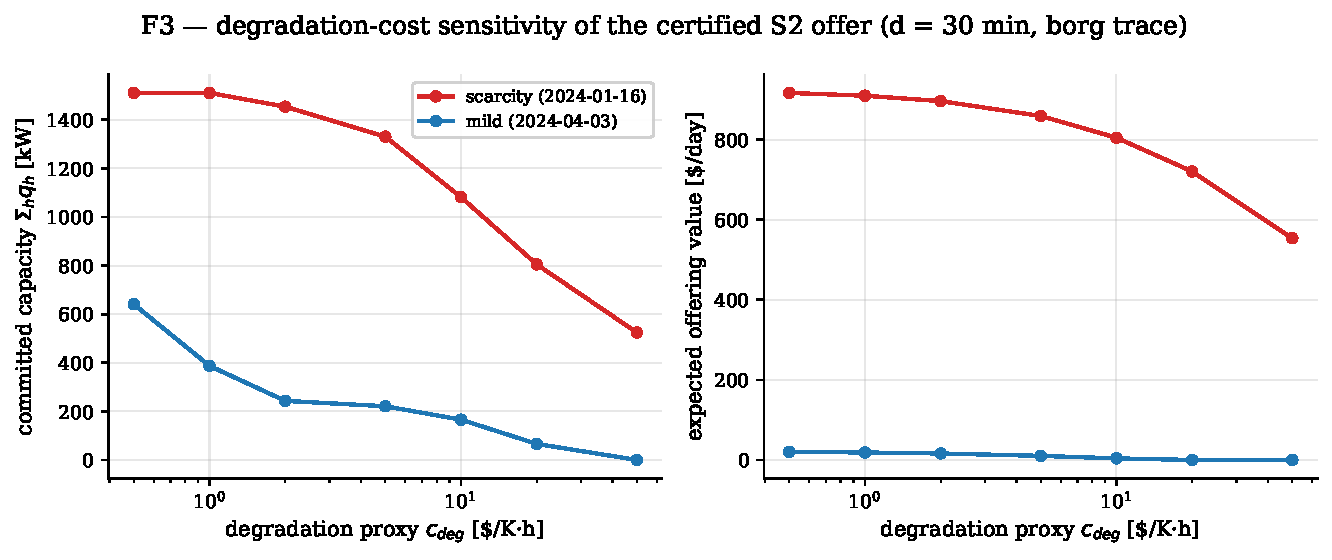
\includegraphics[width=\columnwidth]{../results/phase6/F3_cdeg.pdf}
\caption{Degradation-cost sensitivity of the certified daily commitment
(scarcity vs.\ mild day, $d=30$\,min): monotone contraction; the mild day
exits beyond $c_{\mathrm{deg}}\approx 20$\,\$/K$\cdot$h.}
\label{fig:F3}
\vspace{-3mm}
\end{figure}

\vspace{-3mm}
\subsection{Scope and Limitations}
\label{subsec:limits}

Four modeling commitments bound the claims. (i) The duration $d$ is a product
parameter: thermal inertia is a minutes-scale resource, and the envelope
quantifies how capability decays with $d$; hours-scale products belong to
batteries and workload shifting. (ii) The topology assumes chiller-assisted
heat rejection, so reducing rejection power is always feasible;
free-cooling-dominated plants couple to ambient temperature through a
different mechanism. (iii) Metering is at the cooling plant against an
exogenous baseline (Remark~\ref{rem:baseline}). (iv) Beyond the calibrated
safety set, hardware frequency scaling is the backstop, and the measured
excursions there ($\le 1.6$\,K) are reported rather than assumed away.
Economically, the average value is price-limited: ENCORE captures roughly a
third of the unconstrained ceiling on 2024 ERCOT prices and near-half during
scarcity, so the business case is scarcity participation plus
interconnection optionality~\cite{norris2025rethinking,sb6_2025}, not
baseload arbitrage. The clearest paths to deeper certified offers are
informational and structural: richer operator job schedules (the running-job
forecast is a lower bound on what operators know), duration-layered products,
and affine disturbance feedback in place of the fixed gain.

\vspace{-2mm}
